\graphicspath{{./experiment/}}

\chapter{Experiment}
% {{{
\label{cha:experiment}

\section{Introduction}
% {{{
\label{sec:experiment_introduction}

% TODO: why quantisation again?

The position data to be compressed in our water compression system is floating
point data, however, as an arithmetic encoder is used, the floating point data
will need to be quantised to a specific number of bits.

An appropriate number of bits to use to represent the quantised data will need
to be chosen. Fewer bits used will result in higher compression, but more data
will be initially discarded; while more bits used will result in lower
compression, but the data is stored at higher levels of precision.

To determine the appropriate level of quantisation, an experiment was conducted
to test the perceptually visible effects of quantisation. More simply stated:
how noticable are the effects of quantisation? This will help determine the
appropriate level of quantisation; using the least number of bits, while
maintaining visual similarity to the original data.

Figures \ref{fig:experiment_ballstick4680} and
\ref{fig:experiment_metaballs4680} shows the different quantisation levels for
the ball and stick, and metaballs visualisation techniques respecitvely. The
original unquantised data is on the left, with the four different quantisation
levels; 10 and 8 bit quantisation at the top, 6 and 4 bit quantisation at the
bottom.

\begin{figure}[h!]
  \begin{center}
    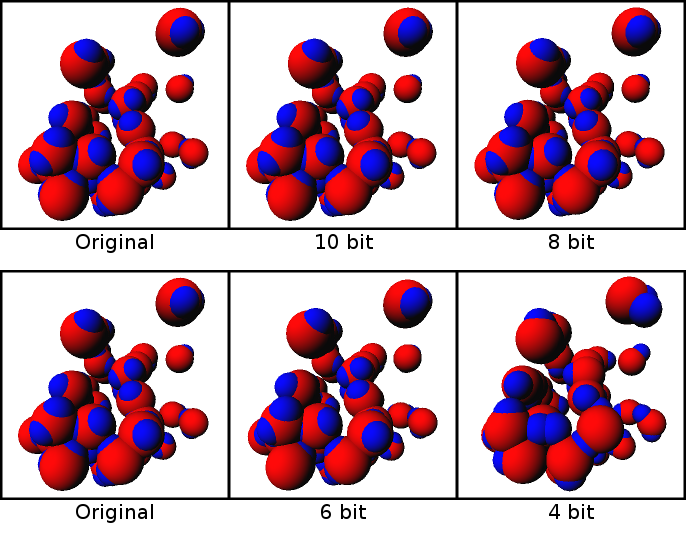
\includegraphics[width=120mm]{ballstick4680}
  \end{center}
  \caption{Ball and stick visualisation showing the different quantisation
  levels}
  \label{fig:experiment_ballstick4680}
\end{figure}

\begin{figure}[h!]
  \begin{center}
    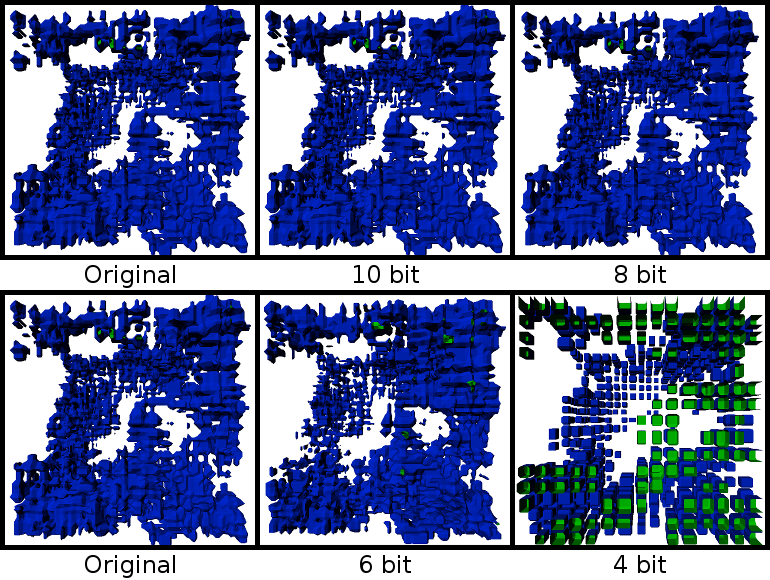
\includegraphics[width=120mm]{metaballs4680}
  \end{center}
  \caption{Metaballs visualisation showing the different quantisation
  levels}
  \label{fig:experiment_metaballs4680}
\end{figure}

Section \ref{sec:experiment_design} details the experiment carried out, while
Section \ref{sec:experiment_results} presents the results and analysis for the
experiment. A final summary and recommendation is presented in Section
\ref{sec:experiment_summary}.

% }}}

\section{Experiment Design}
% {{{
\label{sec:experiment_design}

\subsection{Venue and equipment}
% {{{
\label{sub:experiment_venue}

The participants took part in the experiment one at a time within a closed
room. They watched the data on a monitor, which was connected to a laptop. The
laptop was used to load and display the data. The same laptop was used for all
the experiments:
\begin{itemize}
  \item Processor: Intel Core 2 Duo Processor T6570 2.1GHz
  \item Memory: 2GB DDR2
  \item GPU: Mobile Intel Graphics Media Accelerator X4500 HD
\end{itemize}

% }}}

\subsection{Participants}
% {{{
\label{sub:experiment_participants}

All the partipants were students from the University of Cape Town. Half of the
participants were Science students, with the remaining half consisted of mostly
Commerce and Humanities students.

The only requirement for a participant to take part in the experiment is that
they are not visually impaired. All that is needed is that they are able to
watch and compare two different sets of data (molecular visualisations).

A total of 30 participants took part in the experiment. Most of the experiments
were completed in the first three days (25 of the planned 30), while the
remaining experiments completed over three more days.

% }}}

\subsection{Variables}
% {{{
\label{sub:experiment_variables}

The variables of the experiment are the four different quantisation levels, and
the two different visualiation techniques.

The four quantisation levels tested were:
\begin{itemize}
  \item 4 bit quantisation
  \item 6 bit quantisation
  \item 8 bit quantisation
  \item 10 bit quantisation
\end{itemize}

10 bit quantisation was chosen as the upper quantisation level to test because
beyond 10 bits, the quantisation effects are too minimal to be noticeable. Even
at 10 bit quantisation, the differences are miniscule (see Figure
\ref{fig:experiment_ballstick4680}).

The two visualisation techniques were:
\begin{itemize}
  \item Ball and stick view
  \item Metaballs view
\end{itemize}

At the time of the experiment, there were four datasets available, all of which
were used and randomly selected for the participants.

% }}}

\subsection{Procedure}
% {{{
\label{sub:experiment_procedure}

\begin{enumerate}

  \item The subject will be given a piece of paper explaining the experiment
  and what they are to do.

  \item A random dataset is selected for the participant.

  \item The original unquantised data will be loaded and the subject will be
  allowed to explore and view it.

  \item Thereafter, two different quantised data will be loaded for the subject
  to see.

  \item The original data will the loaded again to remind the participant what
  the original data looked like.

  \item A final two more quantised data will be loaded.

  \item The quantisation levels will be chosen in a random order.

  \item After showing each quantised data, the subject will be asked to compare
  it with the original data, indicating on a scale of 1 to 7, how noticeable the
  differences are: 1 being "Not noticeable" and 7 being "Very obvious".

  \item This procedure will be repeated for a total of 2 visualisation
  techniques, with 2 different datasets each.

  \item The order of visualisation techniques shown will be the same: ball and
  stick, then metaballs.

\end{enumerate}

On average, the participants took 25 minutes to complete the experiment. The
duration of the experiment varied due to the different datasets. Not all the
datasets used were of equal size or length, some datasets required more time to
play from start to finish.

After conducting a pilot experiment, it was decided that the participant should
not be able to rotate and explore the data. Rotating the view makes the data
look very different, this could invalidate the results of the experiment as the
participants will not be able to accurately compare the unquantised and
quantised data.

% }}}

% }}}

\section{Results}
% {{{
\label{sec:experiment_results}

\subsection{Methodology}
% {{{
\label{sub:experiment_methodology}

A series of statistical tests is conducted on the data to determine various
statistical properties.

\paragraph{Shapiro-Wilks Test}
The first test is for normality. Further tests that can be conducted on the
data depends on whether the data is normal or not, thus it is important to
determine the normality of the data. The hypothesis and null hypothesis of the
Shapiro-Wilks Test are: \\ \\
\textbf{Hypothesis:} The data is a normal distribution. \\
\textbf{Null hypothesis:} The data is not a normal distribution.

\paragraph{Friedman Test}
Determining if the datasets have an impact on the perceived differences for a
specific quantisation level needs to be done. However, half of the data does
not form a normal distribution. Hence, non-parametric statistical analysis will
need to be conducted.

If the data is not normal, the Friedman Test can be used to determine if the
factors have a statistically significant impact on the data. For this
experiment, the hypothesis and null hypothesis are: \\ \\
\textbf{Hypothesis:} The datasets used have an impact on the results. \\
\textbf{Null hypothesis:} The datasets do not have impact on the results.

The results from the Friedman Test indicates that the null hypothesis cannot be
rejected, meaning that the datasets do not have a significant impact on the
results. Hence, analysis on the aggregated data can be done; i.e. ignoring
datasets.

\paragraph{ANOVA}
The aggregated data for the different quantisation levels and visualisation
techniques does form a normal distribution. Hence, non-parametric analysis of
the data is not needed.

If the data is normal, then an Analysis of Variance (ANOVA) can be conducted to
determine if the factors have a statistically significant impact on the data.
For this experiment, the hypothesis and null hypothesis are: \\ \\
\textbf{Hypothesis:} Quantisation has an impact on the perceived difference
between the unquantised and quantised data. \\
\textbf{Null hypothesis:} Quantisation does not have an impact on the perceived
difference between the unquantised and quantised data.

\paragraph{Tukey's HSD}
An ANOVA analysis only indicates whether the factors have a significant impact
on the data or not. To compare the factors (the different quantisation levels),
Tukey's HSD (Honestly Significant Difference) test can be used. Tukey's HSD
does pair-wise comparisons of the resulting means for each of the factors,
indicating how similar the results are.

\paragraph{Box and whisker plot}
To graphically depict the differences between the factors, a box and whisker
plot can be used. The effect of the box and whisker plot is similar to Tukey's
HSD in that it is possible to see the individual factors and compare them to
one another.

The results from the tests is presented in Section
\ref{sub:experiment_results}, they are then analysed and discussed in Section
\ref{sec:experiment_discussion}. Following the methodology, the results from
the different datasets is first presented and analysed, followed by the
aggregated results.

% }}}

\subsection{Results}
% {{{
\label{sub:experiment_results}

\subsubsection{Dataset specific}
% {{{
\label{ssub:experiment_results_dataset}

Four datasets were used for the experiment. As there were 30 participants, and
each participant viewed two datasets, each dataset was viewed a total of 15
times.

After performing the Shapiro-Wilks test for each of the dataset specific
results, the null hypothesis could not be rejected for some of the results.
i.e. Some of the results do not form a normal distribution. Appendix
\ref{cha:statsresults} contains a table detailing the test results for all the
separate datasets and quantisation levels. A possibility for why the data does
not form a normal distribution may be due to insufficient sampling. 15 data
points may not be enough to accurately capture the distribution.

As not all the data follows a normal distribution, the Friedman Test was
performed. The results from the test (Appendix \ref{cha:statsresults})
indicates that the null hypothesis cannot be rejected for all the data, i.e.
the different datasets do not have a significant impact on the results. The
only exception to this is for the ball and stick visualisation technique, using
10 bit quantisation.

Since the datasets do not have a significant impact on the results, the results
from individual datasets can be combined. Allowing for a more general analysis
of the results.

Plotting the results on a box and whisker plot (Figures
\ref{fig:experiment_boxwhisker_dataset_ballstick} and
\ref{fig:experiment_boxwhisker_dataset_metaballs}), shows that the results are
quite similar. The largest variations within quantisation levels is for the
metaballs visualisation technique. However, while the results do differ, they
do not contradict each other.

\begin{figure}[h!]
  \begin{center}
    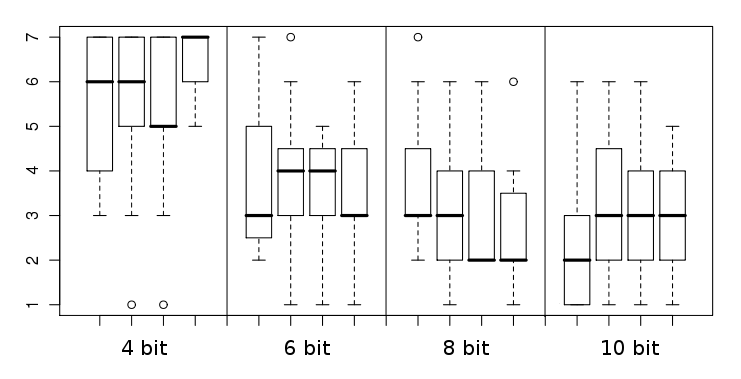
\includegraphics[width=120mm]{boxwhisker_dataset_ballstick}
  \end{center}
  \caption{Box and whisker plot of the different quantisation levels for the
  ball and stick visualisation technique, showing the different datasets}
  \label{fig:experiment_boxwhisker_dataset_ballstick}
\end{figure}

\begin{figure}[h!]
  \begin{center}
    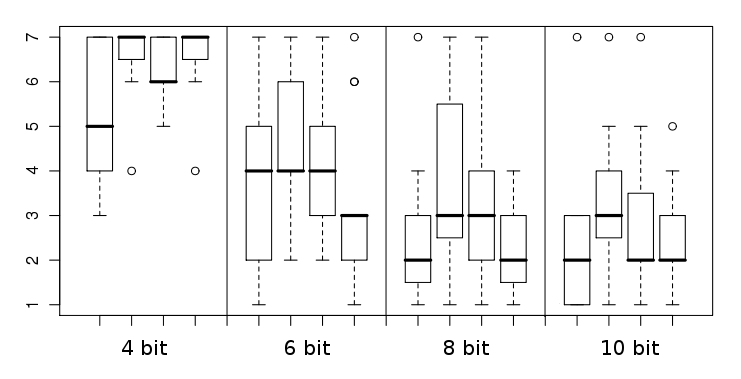
\includegraphics[width=120mm]{boxwhisker_dataset_metaballs}
  \end{center}
  \caption{Box and whisker plot of the different quantisation levels for the
  metaballs visualisation technique, showing the different datasets}
  \label{fig:experiment_boxwhisker_dataset_metaballs}
\end{figure}

% }}}

\subsubsection{Aggregated}
% {{{
\label{ssub:experiment_results_aggregated}

Using the Shapiro-Wilks test for normality on the aggregated data for the ball
and stick, and metaballs visualisation techniques, the null hypothesis of the
Shapiro-Wilks test can be rejected at the 95\% significance level; i.e. the
data is a normal distribution. See Appendix \ref{cha:statsresults} for the
actual test results.

With the data being verfied as a normal distribution, the ANOVA analysis can be
performed. The result from ANOVA analysis indicates that the null hypothesis of
the ANOVA analysis can be rejected at the 99\% significance level, i.e.
quantisation does have a significant perceptual impact. See Appendix
\ref{cha:statsresults} for the actual test results.

Table \ref{tab:experiment_ballstick_tukeyhsd} and
\ref{tab:experiment_metaballs_tukeyhsd} shows the results from performing the
Tukey's HSD analysis on the results from the ball and stick, and metaballs
experiments respectively. The left column shows which quantisation levels are
being compared. For ball and stick, b4 means quantisation using 4 bits, b6 is 6
bit quantisation, b8 and b10 uses 8 and 10 bits respectively. Similarly: m4,
m6, m8 and m10 means quantisation levels using 4, 6, 8 and 10 bits for the
metaballs visualisation technique. The difference between the means is under
the \emph{diff} column, with the lower and upper quartiles in \emph{lwr} and
\emph{upr} respectively. \emph{p adj} indicates how similar the factors being
compared are.

Looking at the \emph{p adj} column, 8 and 10 bit quantisation are very similar.
6 and 8 bit quantisation is also very similary, but the difference is more
noticeable than that between 8 and 10 bit quantisation. 4 bit quantisation is
significantly different from all the other quantisation levels.

Figure \ref{fig:experiment_boxwhisker_all} is a box and whisker plot showing
the different quantisation levels. The ball and stick results are on the left
half of the figure, while the right half is for the metaballs technique. The
figure reflects the data from the Tukey's HSD analysis, 8 and 10 bit
quantisation is similar, 6 and 8 bit less so, and 4 bit quantisation is
different from all the other quantisation levels.

Looking at the box and whisker plot (Figure
\ref{fig:experiment_boxwhisker_all}), the participants rated 4 bit quantisation
as being very different to the original (median rating of 6 and 7), with 6 bit
being different (median rating of 4), 8 and 10 bit quantisation being
moderately different (median rating of 3).

\begin{table}[h!]
  \begin{tabular}{ | l | r | r | r | r |}
  \hline
         &       diff &        lwr &        upr &     p adj  \\ \hline
  b4-b10 &  2.7833333 &  2.0924164 &  3.4742503 & 0.0000000  \\ \hline
  b6-b10 &  0.8000000 &  0.1090830 &  1.4909170 & 0.0159128  \\ \hline
  b8-b10 &  0.2833333 & -0.4075836 &  0.9742503 & 0.7135299  \\ \hline
  b6-b4  & -1.9833333 & -2.6742503 & -1.2924164 & 0.0000000  \\ \hline
  b8-b4  & -2.5000000 & -3.1909170 & -1.8090830 & 0.0000000  \\ \hline
  b8-b6  & -0.5166667 & -1.2075836 &  0.1742503 & 0.2163136  \\ \hline
  \end{tabular}
  \caption{Tukey's HSD test results for the ball and stick visualisation
  technique}
  \label{tab:experiment_ballstick_tukeyhsd}
\end{table}

\begin{table}[h!]
  \begin{tabular}{ | l | r | r | r | r |}
  \hline
         &       diff &        lwr &        upr &     p adj  \\ \hline
  m4-m10 &  3.4833333 &  2.7518209 &  4.2148457 & 0.0000000  \\ \hline
  m6-m10 &  1.2333333 &  0.5018209 &  1.9648457 & 0.0001127  \\ \hline
  m8-m10 &  0.1166667 & -0.6148457 &  0.8481791 & 0.9762546  \\ \hline
  m6-m4  & -2.2500000 & -2.9815124 & -1.5184876 & 0.0000000  \\ \hline
  m8-m4  & -3.3666667 & -4.0981791 & -2.6351543 & 0.0000000  \\ \hline
  m8-m6  & -1.1166667 & -1.8481791 & -0.3851543 & 0.0005950  \\ \hline
  \end{tabular}
  \caption{Tukey's HSD test results for the metaballs visualisation technique}
  \label{tab:experiment_metaballs_tukeyhsd}
\end{table}

\begin{figure}[h!]
  \begin{center}
    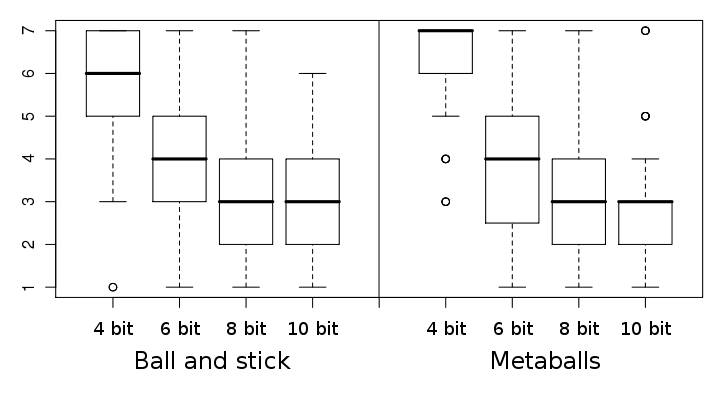
\includegraphics[width=120mm]{boxwhisker_all_both}
  \end{center}
  \caption{Box and whisker plot of the different quantisation levels}
  \label{fig:experiment_boxwhisker_all}
\end{figure}

% }}}

% }}}

% }}}

\section{Discussion}
% {{{
\label{sec:experiment_discussion}

\subsection{Dataset specific}
% {{{
\label{sub:experiment_discussion_dataset}

As mentioned in Section \ref{ssub:experiment_results_dataset}, the Friedman
Test indicates that the different datasets do not have a significant impact on
the results. This means that the perceptually visible effects of quantisation
is similar between datasets.

The effects are not exactly equal due to the size differences in the datasets.
As quantisation produces a limited number of possible values which can be used,
a dataset with large dimensions will have more quantisation error, and thus
more noticeable differences.

However, for datasets with fewer molecules, the bounding box of the data can
shift around as the molecules move.  With more molecules, the bounding box is
more likely to remain still as more molecules will need to move in a certain
direction to shift the shift the bounding box.  As quantisation allocates
values equally across the bounding box, a shift in the bounding box would cause
a corresponding shift of all the values. In the visualisation, this would be
characterised as the entire volume of data moving around. The simulation would
appear ``wobbly''. The wobbling is more noticeable with quantisation using
fewer bits.

In further analysing the data, there is no consistent increase or decrease in
the noticeable difference with regards to datasets.  This may have been as a
result of a number of factors:
\begin{itemize}

  \item participant uncertainty, different participants have their own
  different definitions of ``similar'' and ``different''.

  \item participant bias, participants can be biased towards perceiving
  similarities, or differences, hence skew their results.

  \item the quantisation levels were shown in a random order, this may
  influence the participants short-term memory, and thus impact on the
  perceived differences.

  \item large datasets have greater quantisation errors, but smaller datasets
  ``wobble'', there is thus a visual difference either way.

\end{itemize}

While there are differences as a result of the datasets, the differences are
small and the responses are consistent across datasets.

% }}}

\subsection{Aggregated}
% {{{
\label{sub:experiment_discussion_aggregated}

As the dataset does not have a significant impact on the results, all the
results for a specific quantisation level and visualisation technique can be
combined and aggregated toegher. This allows for a more general analysis on the
effects of quantisation to be done.

The responses from the experiment indicate that 8 and 10 bit quantisation
yields similar results, 6 bit is still similar but less so, while 4 bit being
very different from the original data. This does reflect the effects of
quantisation. As fewer bits are used, exponentially fewer values are available.
10 bits allows for 1024 possible values, but 4 bits only allows for 16 possible
values. See Table \ref{tab:experiment_bitvalues} for a table showing the number
of possible values for each of the quantisation levels.

\begin{table}[h!]
  \begin{tabular}{ | l | r | }
  \hline
  Quantisation level & Number of values  \\ \hline
  4 bit              &               16  \\ \hline
  6 bit              &               64  \\ \hline
  8 bit              &              256  \\ \hline
  10 bit             &             1024  \\ \hline
  \end{tabular}
  \caption{Table showing number of values per quantisation level}
  \label{tab:experiment_bitvalues}
\end{table}

Plotting the means of the quantisation levels (Figure
\ref{fig:experiment_bm_means}) shows that the metaballs visualisation technique
yields more noticeable differences when using fewer bits, than that of ball and
stick. This is especially true at the 4 bit quantisation level.

\begin{figure}[h!]
  \begin{center}
    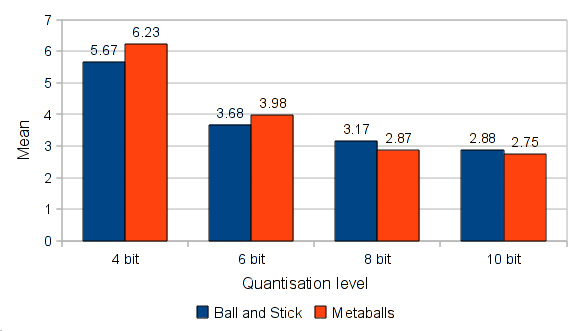
\includegraphics[width=100mm]{bm_means}
  \end{center}
  \caption{Graph showing the mean values of the different quantisation levels}
  \label{fig:experiment_bm_means}
\end{figure}

As the ball and stick visualisation technique shows the individual atoms, this
is why it is easier to see the differences between the original and quantised
data. The spheres are at the actual quantised values, quantisation will result
in the spheres being placed in a different position, hence be easily noticed.

Due to how the metaballs surface is extracted, the quantisation effects are
very noticeable when using fewer bits. As fewer bits are used, there will be
fewer positions for the water molecules. As there are fewer positions for the
water molecules, this will distort the areas of water and non-water. The
resulting extracted surfaces will highlight the quantised positions. See Figure
\ref{fig:experiment_metaballs4680}, the quantised water positions are clearly
visible when using 4 bit quantisation.

The quantised water positions are not as clearly visible when using more bits
as the water molecules are placed more accurately, the water molecules do not
overlap as much.

The metaballs surface is determined by the nearby water molecules, which means
that slight variations in the water molecule positions will not be clearly
reflected on the surface. This would contribute to why the 8 and 10
quantisation levels are so similar.

% }}}

% }}}

\section{Summary}
% {{{
\label{sec:experiment_summary}

The statistical analysis shows that the datasets do not have a significant
impact on the results, meaning that the results between datasets are comparably
similar.

Aggregating the data from the different datasets together, and analysing that
shows that quantisation levels do have a statistically significant impact on
the perceived difference. People are able to perceive the different
quantisation levels.

At quantisation levels that use fewer bits, the metaballs visualisation
technique is rated to be more different than that of the ball and stick
visualisation technique. While the ball and stick ratings for quantisation
levels using more bits is higher; i.e. the difference between the original data
is greater.

As the perceived difference between 8 and 10 bit quantisation levels is minor,
8 bit quantisation is the recommended quantisation level to use. If the data to
be compressed is very large, more bits per quantisation may be needed. However,
for data to be viewed by people, 8 bit quantisation is sufficient.

% }}}

% }}}

